
\chapter{Materials and methodology}\label{method}
% das eher in einleitung
The task of this thesis is to improve semantic segmentation in minimally invasive surgery, in the sense that it is more robust against interferences.
The main interference, that complicates the semantic segmentation is the smoke that occurs when tissue parts are cut with the help of an electrical cutter.
The segmentation is carried out with a segmentation network, which is trained with images from videos of real surgery.\\
The first approach to make it perform better is to artificially translate images with no smoke from the training set into smoked ones.
They are then used in the training of the semantic segmentation network.
The first section \ref{data_pres} of this paper provides a description of the dataset used in this work.
Following that, a general overview of GANs is presented in section \ref{gans_allg}, with specific focus on the variants CycleGAN and StarGAN in section \ref{gan_var_l}. 
Subsequently, the methods to improve the segmentation with I2I translation are proposed in section \ref{seg_improve_gen}.
\section{Data}\label{data_pres}
% \begin{figure}[!htb]
%     \centering
%     \minipage{0.32\textwidth}
%       \includegraphics[width=\linewidth]{./images/f_13075_video_1.png}
%       \caption{A really Awesome Image}\label{fig:awesome_image1}
%     \endminipage\hfill
%     \minipage{0.32\textwidth}
%       \includegraphics[width=\linewidth]{./images/13075_mask_color_video1.png}
%       \caption{A really Awesome Image}\label{fig:awesome_image2}
%     \endminipage\hfill
%     \minipage{0.32\textwidth}
%       \includegraphics[width=\linewidth]{./images/f_26006_video1.png}
%       \caption{A really Awesome Image}\label{fig:awesome_image3}
%     \endminipage
%\end{figure}
\begin{figure}[h]
    \centering
    \subfloat[]{\includegraphics[width=0.45\textwidth]{./images/f_13075_video_1.png}\label{fig:image1}}
    \hfill
    \subfloat[]{\includegraphics[width=0.45\textwidth]{./images/13075_mask_color_video1.png}\label{fig:image2}}
    
    \vspace{1cm}
    
    \subfloat[]{\includegraphics[width=0.45\textwidth]{./images/f_26006_video1.png}\label{fig:image3}}
    \hfill
    \subfloat[]{\includegraphics[width=0.45\textwidth]{./images/f_20051_ss.png}\label{fig:image4}}
    
    \caption[Display of data]{(a) shows an image from the no-smoke domain with the corresponding ground truth segmentation mask (b). 
    (c) shows an image from the heavy-smoke domain, (d) from the slight-smoke domain.}
    \label{example_imgs}
\end{figure}

% \begin{figure}[!htb]
% \minipage{0.32\textwidth}
%   \includegraphics[width=\linewidth]{./images/f_13075_video_1.png}
%   %\caption{A really Awesome Image}\label{fig:awesome_image1}
% \endminipage
% \minipage{0.32\textwidth}%
%   \includegraphics[width=\linewidth]{./images/13075_mask_color_video1.png}
%   %\caption{Here samples from the used data can be seen.}\label{fig:awesome_image3}
% \endminipage\hfill
% \minipage{0.32\textwidth}
%   \includegraphics[width=\linewidth]{./images/f_26006_video1.png}
%   %\caption{A really Awesome Image}\label{fig:awesome_image2}
% \endminipage\hfill
% \label{example_imgs}
% \caption*{On the left, an image from the no-smoke domain with the corresponding ground truth segmentation mask can be seen. 
% The right image shows an image from the heavy-smoke domain.}
% \end{figure}

% aufgeteilt in drei gruppen
\begin{table}[bt]\vspace{1ex}\centering
    \captionsetup{justification=centering}
    \caption[Data description.]{Here the number of used frames per video and domain are shown.
    \label{image_distribution}}
    \begin{tabular*}{12cm}{ll|@{\extracolsep\fill}cccc}
    &&\multicolumn{3}{c}{Images} \\
    && No smoke & Slight smoke &  Heavy smoke \\\hline
    \multirow{6}*{\rotatebox{90}{Videos}}
    & Video 1 &  16,753  & 5,445  & 13,072  \\%\cline{2-6}
    & Video 2 & 46,586  & 9,750 & 7,516  \\%\cline{2-6}
    & Video 3 &  15,508  & 4,920 & 13,752 \\%\cline{2-6}
    & Video 4 &  40,512  & 9,698 & 14,211 \\%\cline{2-6}
    & Video 5 &  23,730  & 6,335 & 6,323 \\
    & Video 6 &  17,762  & 3,145 & 6,473 \\\hline
    \end{tabular*}
\vspace{2ex}\end{table}
% wie viele in den drei gruppen
% dabei nur jeder 25 frame und die weggelassen die zb außerhalb sin
The data used in this thesis comes from six real videos of minimally invasive surgery.
They are recorded at a frame rate of 25 frames per second. 
To be used for image-to-image translation it is also necessary to divide the images into three domains: no-smoke, slight-smoke, and heavy-smoke.
Also, some frames without information about one of the domains, like when the endoscope camera is cleaned, are not used.
This results in 61,347 heavy smoke, 39,293 medium smoke, and 160,851 no-smoke frames. In total, there are 261,491 frames which could potentially be used.
The exact distribution can be seen in Table \ref{image_distribution}.\\
To train an ANN in a supervised way, the data must be annotated, which means the objects that should be segmented have to be marked manually.
For efficiency reasons, only every 25th frame is annotated.
Also, the information gain in directly successive frames is not very high, because the change in the images is marginal.
For this reason and because only every 25th frame is annotated for segmentation, only every 25th frame is used for training.
The important parts of the image are in this case the surgical instruments, which are therefore annotated as segmentation masks.
Example images and a segmentation mask are shown in Figure \ref{example_imgs}.
There are a total of 17 different instruments and therefore 18 classes to be segmented, including the background.
In order to work with this data, the annotated segmentation masks are saved as a two-dimensional matrix with the size equal to the respective image.
For each pixel, the corresponding value in this matrix represents one class.
The class values with the associated surgical instrument meaning are shown in Table \ref{surg_inst}.
\begin{table}[!tb]\vspace{1ex}\centering
    \caption[Surgical instruments]{Display of the surgical instruments with their respective class.
    \label{surg_inst}}
    \begin{tabular*}{6cm}{cc}
    Surgical instrument & Class\\\hline
     Background & 0\\
     Retrieval-Bags & 1\\
     Palpatation-Probe & 2\\
     Needle-Probe & 3\\
     Trokar-Tip & 4\\
     Clips & 5\\
     Clip-Applicator-Tip&6\\
     Suction-Rod Tip& 7 \\
     HFcoag-Probe Tip& 8 \\
     Grasper Tip& 9 \\
     PE-Forceps Tip& 10\\ 
     Scissors Tip& 11 \\
     Drainage& 12 \\
     Blunt Grasper Tip& 13\\ 
     Overholt Tip& 14 \\
     Hook Clamp Tip& 15 \\
     Argonbeamer Tip& 16 \\
     Shaft& 17\\\hline
    \end{tabular*}
\vspace{2ex}\end{table}
% \begin{itemize}
%     \item Background: 0
%     \item Retrieval-Bags: 1
%     \item Palpatation-Probe: 2
%     \item Needle-Probe: 3
%     \item Trokar-Tip: 4
%     \item Clips: 5
%     \item Clip-Applicator-Tip:6
%     \item Suction-Rod Tip: 7 
%     \item HFcoag-Probe Tip: 8 
%     \item Grasper Tip: 9 
%     \item PE-Forceps Tip: 10 
%     \item Scissors Tip: 11 
%     \item Drainage: 12 
%     \item Blunt Grasper Tip: 13 
%     \item Overholt Tip: 14 
%     \item Hook Clamp Tip: 15 
%     \item Argonbeamer Tip: 16 
%     \item Shaft: 17
% \end{itemize}
\clearpage
\section{Generative adversarial networks}\label{gans_allg}
One method to artificially generate data is with the help of Generative Adversarial Networks (GANs). To reach that goal a \acs{gan} is trained with data, that corresponds to the desired output.
Thereby it learns the model distribution, which should resemble the distribution in said data \cite{Goodfellow2020}.
In an image-generation case the probability distribution that the GAN should approximate would be the underlying patterns.\\
The \acs{gan} consists of two different networks, namely the generator and the discriminator.
These two \acsp{ann} are trained simultaneously as described in section \ref{adversariallearning}.
% unsupervised

\subsection{Architecture}
\begin{figure}[!b]
    \begin{center}
     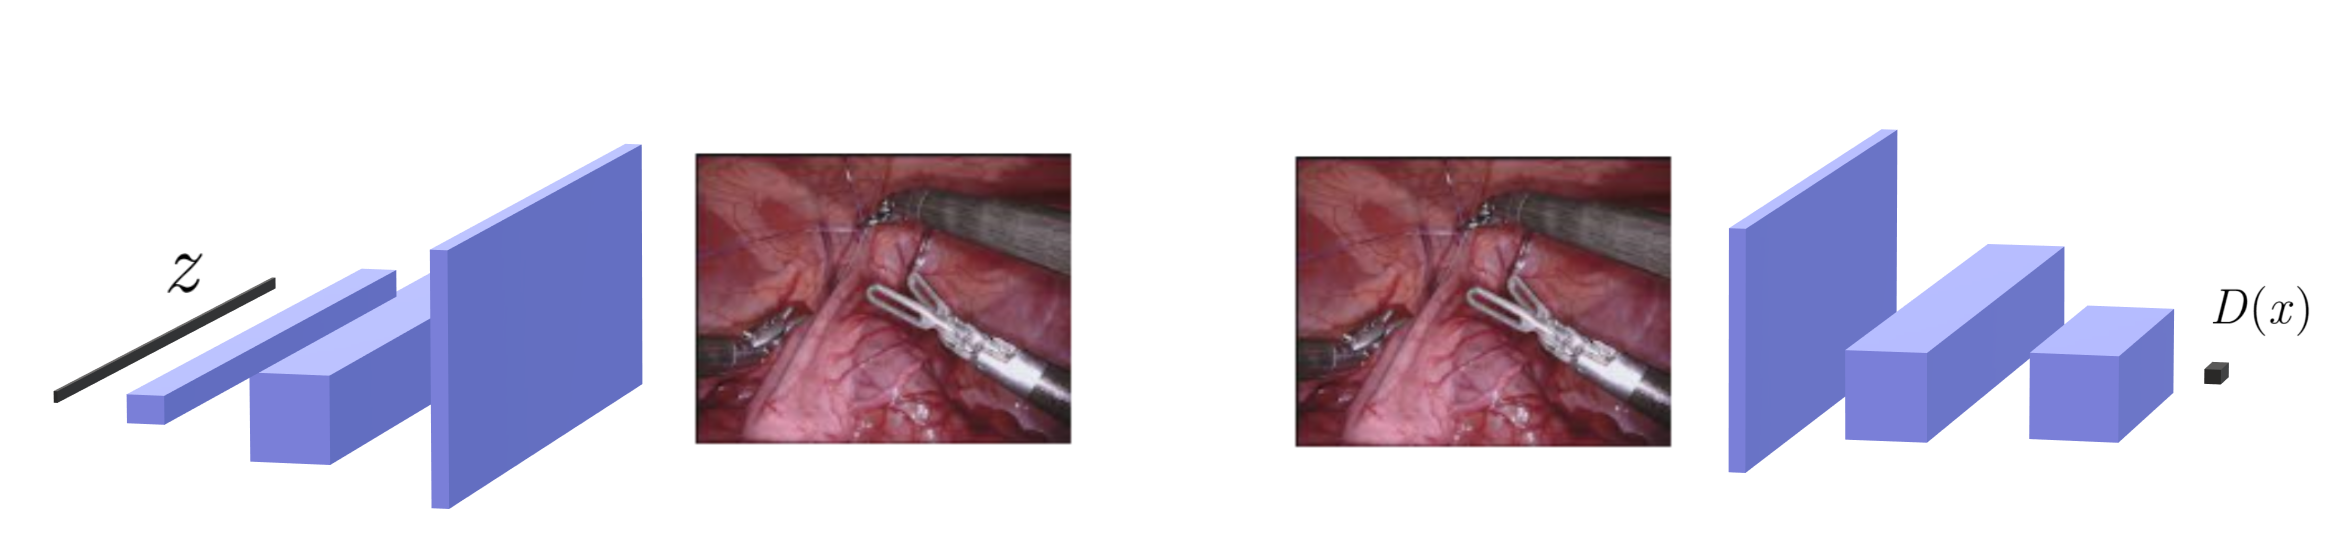
\includegraphics[width=15cm]{./images/gan_conv_image.png}
    \caption[GAN image generation.]{{On the left, an exemplary change in the dimensions of the feature maps in the generator is shown until an image is generated from the sample vector $z$.
        The right side refers to the calculation steps in the discriminator, where the probability $D(x)$, of which distribution the image comes from, is calculated.}\label{gan_conv_image}}
    \end{center}
\end{figure}
The purpose of the generator is to predict an output, that fits the distribution $p_{\text{data}}(x)$ of the training data $x$, through a generator function $G$.
The structure of this process corresponds to the following.
At first, a prior distribution $p_z(z)$ is defined, which is a random distribution to introduce randomness in the model. 
From this, a vector $z$ will be sampled and used as input to the generator function $G(z, \theta^g)$.
$\theta^g$ are the learnable weights of the generator network \cite{Goodfellow2020}.
In image-generation the generator model usually is a \acs{cnn} as described in section \ref{convnetworksection}.
The input vector $z$ will be passed to $G(z, \theta^g)$, where convolution layers will map its input to new feature maps using a suitable kernel dimension.
In this process, the dimensions of the feature maps of the respective layers are modified to finally match the output dimensions of an image.
The changes in the dimensions of the feature maps are shown in Figure \ref{gan_conv_image} exemplarily.
So the random vector $z$ will be processed by $G(z, \theta^g)$ to generate an artificial image as output $G(z)$.\\
%selbst ausgedacht vlt in ... \cite{Aggarwal2021} oder eher hier: Generative Adversarial Networks: An Overview

The task of the discriminator is to decide if a given input $x$ corresponds to the distribution of the training data or to the distribution of the generator.
In the case of image-generation, it determines whether $x$ is an image from the training data or an artificially generated image.
For this, a sample $x$ is passed through the network of the discriminator, which owns the weights $\theta^d$ \cite{Goodfellow2020}.
Therefore the discriminator function $D(x, \theta^d)$ returns a probability $D(x)$, that $x$ derives from the original training data instead of the generated distribution \cite{Goodfellow2014}.\\
In contrast to the generator the input to the discriminator, in this case an image, is downsized while it is processed through the network, as can be seen in Figure \ref{gan_conv_image}.
In the end the output $D(x)$ is often just a single value, which determines the probability.
% deconvolutional

\subsection{Adversarial training}\label{adversariallearning}
\begin{figure}[b]
    \begin{center}
     \includegraphics[width=15cm]{./images/Gan_struktur_cropped.pdf}
    \caption[GAN structure.]{{Schematic overview of how the training of a GAN is structured. The green line thereby represents the weight adjustment depending on $D(x)$.}\label{gan_schematic_fig}}
    \end{center}
\end{figure}
When it comes to the training of a GAN, both the weights of the discriminator and the generator have to be optimized.
Therefore the discriminator is trained to maximize the likelihood of correctly identifying both training data and samples from the artificial data $G(z)$.
The generator on the other hand learns from the results of the discriminator. 
This is done by minimizing $\log(1 - D(G(z)))$. 
In other words, the generator tries to fool the discriminator into making the prediction that a generated image $G(z)$ is an image from the training data.
% minimizing log(1−D(G(z))) is equivalent to minimizing (1−D(G(z)))
The minimum loss for the generator is reached when $D(x)$ will return a probability of one, that its input $G(z)$ is from the original distribution.
This means that the generator is able to successfully fool the discriminator \cite{Goodfellow2014}.
A schematic representation of the training is shown in Figure \ref{gan_schematic_fig}.\\
%Es wird davon ausgegangen, dass D einen a single scalar outputed.
The whole objective function $V(D,G)$ of a GAN can be written as shown in equation \ref{gan_equation}, taken from \cite{Goodfellow2014}:
\begin{equation}
    \min_{G}\max_{D}V(D,G) = \mathbb{E}_{x\sim p_{\text{data}}(x)}[\log D(x)]+\mathbb{E}_{z\sim p_z(z)}[\log(1-D(G(z)))]
    \label{gan_equation}
\end{equation}
The first term in the function $V(G,D)$ represents the expectation $E$ of the logarithm of the discriminator`s output, which stems from samplings $x$ of the training data $p_{\text{data}}(x)$.
In other words, the log-likelihood that the discriminator assigns the real sample $x$ to being an original sample.
The expectation hereby stands for calculating the average value of its operand for all samples of $x$.
This term is responsible for training the discriminator to identify real samples.
The second summand is the expected value of one minus the logarithm of the discriminator`s output $D(x)$ on generated data samples $G(z)$, which is the likelihood that the discriminator assigns the generator's output $G(z)$ to being a fake sample.
Hereby $z$ is a sample from the random distribution $p_z(z)$.\\
The function $V(D,G)$ can be seen as an adversarial loss because the generator $G$ and the discriminator $D$ should either minimize or maximize the value function $V(G,D)$ respectively.
This can be understood as playing a two-player min-max game against each other, where the networks have an opposing goal in the training process.\\
In the training of the basic GAN first, the weights of the generator are fixed and the discriminator is trained a previously defined number of times while maximizing the adversarial loss, so it makes better predictions of which distribution the sample comes from.
Then just the generator is trained and learns to adjust its generation output to correspond more to the distribution $p_{\text{data}}(x)$ of the training data through minimizing the objective function.
Therefore the discriminator performs worse because the generated samples are closer to the training distribution.
This process will be performed in an alternating way until the global optimum is found.
This is the case, when the distribution, that was learned from the generator, is equal to the real distribution $p_{\text{data}}(x)$ \cite{Goodfellow2014}.\\
In practice, this training process is not complex and most of the time an exact optimum cannot be found.
Instead, the models are trained until they converge and reach a stable equilibrium, where both models perform quite well.  
But also reaching this state can be compromised by different error sources.\\
Firstly the two networks can fail to converge, which means they don't reach a stable equilibrium of their losses.
So they can not play the min-max game effectively and do not reach the desired optimum.
If the hyperparameters are not set suitably, the generator, and discriminator won't balance themselves out and one of the networks will overpower the other.
That means that either the generator overfits the data and the discriminator can't learn to differentiate between the real and the fake input or the discriminator gets too good too fast and can't be fooled by the generator. 
Therefore the generator can not effectively learn how to generate an output that is close to the training distribution \cite{Creswell2018}.\\
Another problem is called mode collapse. 
This occurs when the generator learns a small set of outputs, that are all similar for different inputs.
But these results happen to be appropriate to trick the discriminator. Because of this, the GAN does not further adjust its generation process \cite{Creswell2018}.
If such a failure mode can be witnessed, an adjustment of the hyperparameters or a change in the structure of the network is necessary.

\section{Gan variants}\label{gan_var_l}
In this chapter, the the I2I translation networks CycleGAN and StarGAN are presented. 
Both networks will be described in detail, outlining their key characteristics and properties.
\subsection{Cycle GAN}\label{cyclegan}
The translation of images from the not smoked domain to the heavy smoked domain could help the segmentation network make more accurate predictions.
Therefore an image to image translation network can help in this task.
The goal of image translation is to learn the mapping of one image domain to another.
This is usually done using aligned image pairs.
An aligned image pair, for example, would be an image from the exact same position at day and at night.
But this kind of paired data is hard to acquire.
In the case of mapping medical images from a no smoke to a heavy smoke domain, it is not feasible to have the same images available with every instrument and organ in the same place while having smoke present in one and not the other.
Therefore an image translation without the need for aligned image pairs should be used.\\
It is also necessary that specific features that are not related to the smoke stay the same because the labeled segmentation masks should be used for training the segmentation network paired with the generated images.
Otherwise, a network, that is trained on the generated data, would learn false information if for example the appearance of surgical instruments is altered during the translation process.
An image to image translation model that can perform such a task is the CycleGan architecture proposed by Zhu et al. \cite{Zhu2017}.\\
The data here is also used in pairs, but each of them just has to belong to one of the domains, of which the mapping should be learned.
The idea is to use two generators and two discriminators, one for each domain.\\
The generator works in a similar way as in the traditional GAN structure, but it does not sample a random vector for generation.
Instead, it uses an encoder-decoder-like structure to first extract features from an image that should be translated into another domain.
This is done with three convolutional layers.
The first one has a kernel size of 7$\times$7 and stride one, to capture larger features from the image, followed by a convolution with a 3$\times$3 kernel and a stride of two.
Thereby the spatial dimensions of the input feature maps are reduced while the number of feature maps is increased.
The number of filters used from the first to the last convolution layers are: 64, 128, 256.
This way the generator can learn a more abstract representation of the features.\\
After each of those layers instance normalization and a ReLU activation function is used.
Instance normalization calculates the mean and variance for each input in the batch and normalizes them based on these values.
This may improve the performance of image-generation networks \cite{Ulyanov2016}.
The ReLU serves the purpose of introducing sparsity by zeroing all values below zero and therefore avoiding saturation in the network \cite{Sharma2020}.\\
Due to the choice of the number of filters the downsampling results in 256 feature maps, which are then passed to the residual blocks.
As the image size exceeds $256\times256$, nine of them are used, as stated in \cite{Zhu2017}.
These residual blocks contain two 3$\times$3 convolution operations are also followed by ReLU and instance normalization.
The purpose of the residual blocks is to learn the mapping of the feature maps from one domain to the other.\\
After processing through these residual layers, the features are upsampled with the transposed convolution operations corresponding to the two downsampling operations.\\
Then a last convolution operation with kernel size 7$\times$7 and a stride of one is used to generate an output with the same dimension as the input image.
Tangens hyperbolicus (tanh) is used to map the values in the output to the range of [-1, 1], so that it can be scaled to the range of pixel values [0, 255] without outliers.
The change in the feature dimensions of the individual steps in the generator can be seen in Figure \ref{cycle_gen_fig}.
\begin{figure}[bt]
    \begin{center}
     \includegraphics[width=15cm]{./images/gen_cycle.drawio.pdf}
    \caption[CycleGAN generator.]{{Visualization of the modifications regarding the feature maps in the generator.
    The green blocks indicate convolution operations, the red one represent residual blocks, and transposed convolution operations are visualized as blue blocks.
    The dimensions of the output are equal to those of the input image.
    Also, the changes in the height and width of the features depending on the size n of the input image are shown.
    }\label{cycle_gen_fig}}
    \end{center}
\end{figure}
The goal of the discriminator is to distinguish between generated images and those originating from the original dataset.
But instead of downsampling the input images to one value, here a PatchGAN architecture is used, as described in \cite{Isola2016}.
Hence the discriminator returns a two-dimensional matrix with a prediction in each entry.
The entries correspond to a certain area of the image and therefore the discriminator makes a prediction for each area of the image.\\
This is done by applying four 4$\times$4 convolution-InstanceNorm-LeakyReLU blocks, with the stride of the convolutions being two.
The number of filters used is from the first to the last convolution: 64, 128, 256, 512.
LeakyReLU is a variation of ReLU but instead of mapping negative values to 0, it multiplies them with a small constant, to allow non-zero gradients for backpropagation \cite{Sharma2020}.
Instance normalization is skipped for the first layer and the output of the area patches is calculated using a convolution, which combines the 512 feature maps into one output dimension.
The resulting values of the output are mapped to a value range between zero and one through a sigmoid function, indicating if the individual patches are from the generator (close to zero) or from the original data (close to one).\\
The described structure will produce an two-dimensional matrix with the output dimensions $\text{height}_{\text{input}}/2^4 \times \text{width}_{\text{input}}/2^4$, due to four convolutions with stride two.
Each entry thereby represents the discriminator's predictions for the corresponding area in the image.
It is to be noted, that the number of patches is determined through the convolution layers.
The more patches the more accurate the discriminator is but also more resource intensive.
As shown in \cite{isola2017image} a good tradeoff is achieved around a number of 70$\times$70 patches.
The process of how the discriminator calculates a prediction for an input image is shown in Figure \ref{cycle_disc_fig}.
Also, it ought to be remarked that a reflection padding of one is used in the first convolution of the generator and the discriminator, which means mirroring the border pixels of the images to mitigate errors in the edges of the image.\\
\begin{figure}[bt]
    \begin{center}
     \includegraphics[width=10cm]{./images/discriminator.drawio.pdf}
    \caption[CycleGAN discriminator.]{{Visualization of the modifications regarding the feature maps in the discriminator.
        The last convolution transforms the feature maps into the predictions for the corresponding areas in the image.
        Also, the changes in the height and width of the features depending on the size n of the input image are shown.
    }\label{cycle_disc_fig}}
    \end{center}
\end{figure}
To make the four networks work together following training structure is used, as proposed by Zhu et al. \cite{Zhu2017}.\\
There are two of the described generators and discriminators, one for each domain.
A generator $G_A$ is responsible for mapping images from domain $B$ to domain $A$ and one $G_B$ for the opposite case.
To train both of them to produce an output for the desired domain the discriminator networks $D_A$ and $D_B$ are used to create an adversarial loss like the one that is used in the objective function described in \ref{adversariallearning}:
\begin{equation}
    \mathcal{L}_{\text{adv}}(G_B, D_B, A, B) = \mathbb{E}_{b\sim p_{\text{data}}(b)}[\log D_B(b)]+\mathbb{E}_{a\sim p_{\text{data}}(a)}[\log(1-D_B(G_B(a)))]
    \label{adv_loss_cycle}
\end{equation}
This loss is further denoted as $\mathcal{L}_{\text{adv}}(G_B,D_B,A,B)$ for the adversarial loss of the generator $G_B$ and the discriminator $D_B$ for translating images from domain $A$ to $B$.
$\mathcal{L}_{\text{adv}}(G_A,D_A,B,A)$ would be the denotation for the other neural networks in the translation form $B$ to $A$.\\
It is also necessary that features that are not related to the specific domains remain the same in the translation process.
This is ensured by the cycle consistency loss.
The idea behind the cycle consistency loss is that if the generators $G_{A}$ and $G_{B}$ successfully learn the translation between the two domains, then applying for example $G_B$ to an image of $A$ to generate an artificial image of domain $B$ and then applying the other generator $G_A$ to it, it should result in a reconstructed image of domain $A$.
This reconstructed image should be close to the original input from $A$.
The Cycle consistency loss ensures consistent image-generation in CycleGAN by preserving the relevant information from the original input images.
It is defined as follows:
\begin{equation}
    \mathcal{L}_{\text{cyc}}(G_A, G_B) = \mathbb{E}_{a\sim p_{\text{data}}(a)}[\Vert G_A(G_B(a)) - a\Vert_1] + \mathbb{E}_{b\sim p_{\text{data}}(b)}[\Vert G_B(G_A(b)) - b\Vert_1]
\end{equation}
Hereby $\Vert G_A(G_B(a)) - a\Vert_1$ denotes the L1 norm of the cycled reconstruction image $G_A(G_B(a))$ minus the original image $a$.
The L1 norm, also known as Manhatten distance, sums up the absolute values of its input, which in this case results in an absolute difference between the two images.
$\mathbb{E}_{a\sim p_{\text{\text{data}}}(a)}$ denotes the expected value of the L1 norm over the data distribution $p_{\text{data}}(a)$, which means calculating the average value of the L1 norm for all samples of $a$.
%evtl. Expectation formula
% evtl L1 norm formel
This goes for both generators, respectively.
The mentioned losses are then combined to the total objective of the CycleGAN:
\begin{equation}
    \mathcal{L}(G_A, G_B, D_A, D_B) = \mathcal{L}_{\text{adv}}(G_A,D_A,B,A) + \mathcal{L}_{\text{adv}}(G_B,D_B,A,B) + \lambda \mathcal{L}_{\text{cyc}}(G_A, G_B)
    \label{objective_cyclegan}
\end{equation}
The $\lambda$ is hereby a choosable parameter, that adjusts the influence of the cycle consistency loss.
Because it is trained in an adversarial way the following equation has to be solved to get optimal generators $G_A^\ast$ and $G_B^\ast$:
\begin{equation}
    G_A^\ast, G_B^\ast = \text{arg} \underset{G_A, G_B}{\min}\underset{D_A, D_B}{\max}\mathcal{L}(G_A, G_B, D_A, D_B)
\end{equation}
This means finding the configurations $arg$ of the generators which minimize the loss function $\mathcal{L}(G_A, G_B, D_A, D_B)$, while at the same time the configuration of the discriminators should maximize this loss.
As described in section \ref{adversariallearning} this results in a min-max game, where both of the network pairs are trained in an alternating way.
This process is done until the generator and discriminator models converge to a stable state and no longer improve significantly with further training.
A schematic interaction of the individual networks can be seen in Figure \ref{cycle_gan_fig}.\\
\begin{figure}[bt]
    \begin{center}
     \includegraphics[width=15cm]{./images/CycleGan.drawio.pdf}
    \caption[CycleGAN structure.]{{Here the interaction of the individual networks in a CycleGAN training can be seen. 
    For the cycle consistency loss an image from domain $A$ is fed into the generator $G_B$ to generate an artificial image of domain $B$.
    This is used as input for the generator $G_A$ to generate a reconstructed image, which is compared to the original input with the cycle consistency loss, indicated by the black arrows.
    This process is also done for the images from domain $B$, but is not shown in the figure for the sake of clarity.
    The black dotted line shows the generation of an artificial image of domain $B$ which is given to the discriminator $D_B$ with original input from domain $B$ for the adversarial loss.
    This process is also executed for domain $A$ shown with the yellow dotted line. 
    }\label{cycle_gan_fig}}
    \end{center}
\end{figure}
Further adjustments that are made for a more stable training are to change the negative log-likelihood objective in the adversarial loss to a least-squares loss\cite{Zhu2017}.
Hereby the least squares loss can be understood as minimizing the mean squared error (MSE) error of the prediction.
\begin{equation}
    \text{MSE} = \frac{1}{n} \sum_{i=1}^{n} (y_i - \hat{y}_i)^2
\end{equation}
To implement this with a PatchGAN architecture the flattened output patches of the discriminator for a generated image $G_B(a)$ can be compared to a vector of the same length with ones in the case of training the generator.
This is because the training of the generator aims to make the discriminator falsely predict one for a generated image $G_B(a)$.
So the resulting value of the comparison of the prediction of a generated image and the vector with ones is to be minimized to maximize the adversarial loss.
For this comparison, the MSE is used.
Here $y_i$ is the vector with ones, $\hat{y}_i$ is the predicted patch value, and $n$ is the number of patches. 
It calculates the average squared difference between the vector and the predicted values.\\
In the case of training the discriminator the output of itself for a generated image should be zero, therefore the vector with ones is changed to a vector with zeros.
For an image of the original data one should be predicted and therefore the vector can remain being filled with ones before the mean square error is applied.
This way the MSE can be minimized during the whole training, while the comparison vector decides if the adversarial loss is minimized or maximized.\\
Also, there is the option to introduce yet another loss, called identity loss \cite{Zhu2017}.
The idea is to make the generator generate nearly the same image as the input if it is provided already in the target domain.
This loss can be defined as:
\begin{equation}
    \mathcal{L}_{\text{identity}}(G_A, G_B) = \mathbb{E}_{a\sim p_{\text{data}}(a)}[\Vert G_A(a) - a\Vert_1] + \mathbb{E}_{b\sim p_{\text{data}}(b)}[\Vert G_B(b) - b\Vert_1]
\end{equation}
Here the mean absolute difference between the output of the generator $G_A(a)$ that maps to domain $A$ and its input $a$ is calculated with the L1 norm $\Vert \cdot \Vert_1$.
The expectation of this term is calculated and summed up with the output of the same procedure for domain $B$, which will ensure an identity mapping if the input is already in the desired domain.
This loss is multiplied with a choosable parameter to determine its influence in the general loss and added to the total objective in formula \ref{objective_cyclegan}.

An additional adjustment is the use of a buffer to mitigate model oscillation.
This strategy proposed by Shrivastava et al. \cite{Shrivastava2016} involves updating the discriminators using a buffer of previously generated images instead of the ones generated directly before. 


\subsection{StarGAN}\label{star_gan}
StarGan is also an image-to-image translation model based on the GAN architecture proposed by Choi et al.\cite{choi2018stargan}.
It can perform multi-domain translation with a single generator, meaning it can not only translate images from one domain to another, but to multiple domains.
Additionally, the domains, also referenced as styles, can be combined to generate an output, that has the characteristics of different domains.
The main idea is to train the single generator with so-called domain label conditioning. %Zitat
Hereby information about the target domain is given to the generator in the translation process.\\
The following structure of the StarGAN is proposed by Choi et al.\cite{choi2018stargan}.
The structure of the generator in StarGAN is identical to the one used in CycleGAN.
The difference lies in the fact, that the input image of the generator is concatenated with a domain matrix, which serves as information about the domain the image should be translated to.
So assuming there are $n$ possible target domains, $n$ more layers of the dimensions $\text{height}_{\text{image}} \times \text{width}_{\text{image}}$ are attached to the image.
Each of these layers is either completely filled with ones or zeros, depending which domain serves as target for the translation.
So the first layer that is concatenated with the input represents the first domain, the second the second domain, and so on.
\begin{figure}[b]
    \begin{center}
     \includegraphics[width=5cm]{./images/Star_gan_gen_input.drawio.pdf}
    \caption[Domain concatenation StarGAN]{{Here the concatenation of the domain matrix with the input image can be seen. The result is the input for the generator.
    }\label{star_gan_input}}
    \end{center}
\end{figure}
This concatenation is shown in Figure \ref{star_gan_input}.
The concatenated input is given to the generator, which produces an image just like in the CycleGAN architecture.
This way the generator gets the information, to which domain he should translate the input image.
It is to be noted, that the domain matrix is not one hot encoded, so more than one layer can include ones to translate an image to different domains at once.
Also when dealing with translation with multiple domains this domain label conditioning allows the usage of only one generator.
Whereas otherwise, a separate generator would be necessary like in the CycleGAN, where for the translation between two domains two generators are used.\\
The discriminator is also based on a PatchGAN, but with a slightly different structure.
This is because it not only has to predict the distribution of which the input is coming from but also has to predict the source domain of its input.
It is structured as follows.
The input layer of the discriminator is a 4$\times$4 convolution with stride two, 64 filters, and a padding of one followed by a LeakyReLU.
In the hidden layer, there are five more convolutions of the same structure, but with a filter dimension that grows by two with each layer, which results in the following number of filters in this order: 128, 256, 512, 1024, 2048.
Each of those is also followed by a LeakyReLU.
The output layer is divided into two parts.
Firstly as in the CycleGAN, the outputs of the hidden layer are convoluted with a 3$\times$3 kernel, stride of one, and padding one.
This will generate prediction patches, that indicate the authenticity of an area in the input image.
The prediction of the discriminator regarding the origin of the input image is denoted as $D_{\text{src}}$.\\
Secondly, a convolution with $n$ filters for each domain in the specific case is applied to the output of the hidden layer.
The kernel size of this convolution is calculated as $\text{height}_{\text{image}}/2^k \times \text{width}_{\text{image}}/2^k$, whereby $k$ denotes the number of downsampling convolution operations performed beforehand.
In the explained case this would be six resulting from the input and hidden layer.
This output is a vector of length $n$, whereby each entry represents a prediction for the corresponding domains that are present in the input image.
The order of its entries is the same as for layers of the domain matrix concatenation in the generator.
This prediction is further denoted as $D_{\text{dom}}$.\\
To train the StarGAN, different loss functions are needed as proposed by Choi et al. \cite{choi2018stargan}.
To ensure a realistic generation of the images an adversarial loss is used.
Therefore the adversarial loss in the StarGAN for a sample distribution $p_{\text{data}}(x)$ is:
\begin{equation}
    \mathcal{L}_{\text{adv}} = \mathbb{E}_{x\sim p_{\text{data}}(x)}[\log D_{\text{src}}(x)]+\mathbb{E}_{x\sim p_{\text{data}}(x), d}[\log(1-D_{\text{src}}(G(x, d)))]
    \label{adv_loss_star}
\end{equation}
It works the same way as described in section \ref{adversariallearning}, where the goal of the generator $G$ is to minimize this loss whereas the discriminator $D$ tries to maximize it. 
The only difference is that the generator is conditioned on the target domain $d$ and also the expectation $\mathbb{E}_{x\sim p_{\text{data}}(x), d}$ is calculated for the samples $x$ with respect to the chosen target domain $d$.
However, because there is only one generator and discriminator the correct prediction and translation of the image domain is also to be learned.
For training the discriminator to identify the correct domain, the true domain class loss $\mathcal{L}_{\text{dom}}^t$ is defined as:
\begin{equation}
    \mathcal{L}_{\text{dom}}^t = \mathbb{E}_{x\sim p_{\text{data}}(x), d^\prime}[-\log D_{\text{dom}}(d^\prime|x)]
    \label{loss_dom_true}
\end{equation}
This true domain class loss calculates the expectation of the negative log probability of the original domain $d^\prime$ being predicted by the discriminator for an input image $x$.
Therefore when minimizing this loss the probability of the correct prediction of the true domain will rise.\\
Additionally, the generator should learn to translate an image $x$ to the domain $d$, on which it is conditioned to.
The probability of how correctly the generator has mapped the image to the right domain is decided through the discriminator, which makes a prediction of the domain of the image. 
This is ensured through the conditioned domain class loss:
\begin{equation}
    \mathcal{L}_{\text{dom}}^f = \mathbb{E}_{x\sim p_{\text{data}}(x),d}[-\log D_{\text{dom}}(d|G(x,d)]
    \label{loss_dom_false}
\end{equation}
Here the negative log probability of the conditioned domain $d$ being predicted by the discriminator for a generated image $G(x,d)$, which is conditioned with $d$, is calculated.
Of this probability, the expectation is formed over the samples from $p_{\text{data}}(x)$ with respect to the target domain $d$.
This way the generator is made to generate images in a domain, which is predicted correctly by the discriminator.\\
Furthermore a reconstruction loss is used, which should help to preserve the content in the image translation process that is not related to the target domain.
This is similar to the cycle consistency loss in the CycleGAN, but has to be implemented differently because there is only one generator. 
For this, an image $x$ is first translated to a target domain $d$ with the generator.
The output of this is again fed into the generator but conditioned to the original domain $d^\prime$ of the image, which should result in a reconstruction of the original image.
The values of the reconstruction image are subtracted from the values of the original image and from this in turn the L1 norm is calculated, which results in the absolute difference between the images.
If this difference is minimized, the reconstruction image is closer to the original, and therefore the generator produces an image that has similar characteristics as the input.
It can be written as follows:
\begin{equation}
    \mathcal{L}_{\text{rec}} = \mathbb{E}_{x\sim p_{\text{data}}(x),d,d^\prime}[\Vert x - G(G(x,d),d^\prime)\Vert_1]
    \label{loss_reconstruction}
\end{equation}
The presented loss functions are combined to the total objective of the discriminator $\mathcal{L}_D$ and for the generator $\mathcal{L}_G$:
\begin{equation}
    \mathcal{L}_D = -\mathcal{L}_{\text{adv}} + \lambda_{\text{dom}}\mathcal{L}_{\text{dom}}^t 
\end{equation}
\begin{equation}
    \mathcal{L}_G = \mathcal{L}_{\text{adv}} + \lambda_{\text{dom}}\mathcal{L}_{\text{dom}}^f + \lambda_{\text{rec}}\mathcal{L}_{\text{rec}}
\end{equation}
The adversarial loss $\mathcal{L}_{\text{adv}}$ is hereby negated for the discriminator, so if it is minimized the included losses are maximized.
The $\lambda$ parameters hereby are selectable to determine the influence of the individual losses.\\
During the training process, the target domain $d$ is chosen randomly, to ensure that all domains are covered.
\begin{figure}[bt]
    \begin{center}
     \includegraphics[width=10cm]{./images/star_gan.drawio.pdf}
    \caption[Training process StarGAN]{{Visualization of the training process of the StarGAN architecture.
    The original image is translated into a new domain. Then it is again translated to the original domain to create the reconstruction image, which is used for the reconstruction loss.
    Both the original and the translated image are used as input for the discriminator, which produces the probability of the origin $D_{\text{src}}$ to calculate the adversarial loss $\mathcal{L}_{\text{adv}}$.
    The discriminator also makes a prediction of the domain origin $D_{\text{dom}}$ of the translated and the original image, which is used for the true domain loss $\mathcal{L}_{\text{dom}}^t$ and the fake domain loss $\mathcal{L}_{\text{dom}}^f$.
    }\label{star_gan_training}}
    \end{center}
\end{figure}
The training process is visualized in Figure \ref{star_gan_training}.
To improve the training of the StarGAN, Choi et al. \cite{choi2018stargan} use an improved version of the adversarial loss of the Wasserstein GAN introduced by Gulrajani et al. \cite{Gulrajani2017}.
The idea of the original Wasserstein GAN as proposed by Arjovsky et al. \cite{Arjovsky2017} is to measure the distance between the real data and generated data for the adversarial loss.\\
The improved version of the adversarial loss used in StarGAN is an extension of the Wasserstein GAN's objective that enforces the Lipschitz continuity constraint using gradient penalty.
Enforcing the Lipschitz continuity constraint means that a function, in this case the discriminator, has to be Lipschitz continuous, which is defined for a function $f: \mathbb{R}^n \rightarrow \mathbb{R}^m$ on $X\subseteq\mathbb{R}^n$, as shown in equation \ref{lip_const}, taken from \cite{Fazlyab2019}:  
\begin{equation}\label{lip_const}
    \Vert f(x) - f(y) \Vert \leq L\Vert x - y \Vert \forall x,y \in X
\end{equation}
It states that the absolute difference between the function outputs $f(x)$ and $f(y)$ for any points in $X$ is not greater than a constant $L$ multiplied by the absolute difference between the input points $x$ and $y$ \cite{Fazlyab2019}.
Here $L$ is the Lipschitz constant, which denotes how fast the function can change while remaining Lipschitz continuous.
So enforcing the Lipschitz continuity constraint on the discriminator ensures that its output does not change too rapidly and thus helps stabilize the training process.
This is done by adding a gradient penalty to the adversarial loss, which is changed to the Wasserstein distance.
This results in an improved adversarial loss of: 
\begin{equation}
    \mathcal{L}_{\text{adv}} = \mathbb{E}_{x\sim p_{\text{data}}(x)}[D_{\text{src}}(x)]-\mathbb{E}_{x\sim p_{\text{data}}(x), d}[D_{\text{src}}(G(x, d)))] - \lambda_{\text{gp}}\mathbb{E}_{\hat{x}\sim p_{\text{data}}(\hat{x})}[(\Vert\nabla_{\hat{x}}D_{\text{src}}(\hat{x})\Vert_2 -1)^2]
    \label{impr_w_loss}
\end{equation} 
It is to be noted that when using this improved verion the discriminator should not have a sigmoid activation function to make a prediction of the image origin.
Instead, the raw values of the last convolution are used as a score, which is higher for real images and lower for generated images.
In the adversarial loss, seen in equation \ref{impr_w_loss}, the distance between the generated and original images is calculated as the difference of the scores of the original $D_{\text{src}}(x)$ and the generated images $D_{\text{src}}(G(x, d))$, by subtracting the expectations of the latter from the first.
To calculate the gradient penalty the interpolated point $\hat{x}$ is created through sampling between a real and a generated image.
The sampling is done in a straight line, which can be done using the following equation using a random number $\alpha \in [0, 1]$:
\begin{equation}
    \hat{x} = \alpha x + (1 - \alpha)G(x,d)
    \label{interpolated}
\end{equation}
Then the gradient $\nabla_{\hat{x}}D_{\text{src}}(\hat{x})$ of the discriminator with respect to the interpolated point $\hat{x}$ is calculated.
Finally, the gradient penalty is computed as the mean squared difference between the norm of gradients and one.
This gradient penalty is multiplied by a choosable lambda value $\lambda_{gp}$, which determines the influence on the adversarial loss.
The adversarial loss from equation \ref{adv_loss_star} is replaced by this loss.

%evtl. training with different datasets -> mask vector
%kein reflection padding
\section{Improving semantic segmentation}\label{seg_improve_gen}
\subsection{Augmenting data with artificial smoke images}
The initial situation is as follows: there are more frames in the no-smoke domain than in the heavy-smoke domain in all videos.
In order to improve the segmentation network, the ratio of no-smoke to heavy-smoke frames is adjusted during training.
First, the original ratio between the two domains is calculated. 
Then, this ratio is adjusted to create a predetermined ratio of the two domains, for example both domains should have an equal amout of images.
This is done by replacing the frames of the no-smoke domain with the same frames that have been translated into the heavy-smoke domain by an I2I translation network.
The images, which are replaced to obtain the predefined ratio, are chosen randomly each epoch.
With this setup, the segmentation network is trained in a usual way, but with an information gain for the heavy-smoke domain.
\subsection{GenSegNet}
\begin{figure}[b]
    \begin{center}
     \includegraphics[width=14cm]{./images/seg_gen_pdf.pdf}
    \caption[Training structure GenSegNet.]{{Adversarial training structure of the CycleGAN and the segmentation network in GenSegNet. The dotted lines represent the backpropagation to the individual networks.
    }\label{seg_gen_train}}
    \end{center}
\end{figure}
In this section, we propose a method to integrate the segmentation in the generation process and then use in turn the generation to improve the segmentation, called SegGenNet. 
Thereby the translation of images from the no-smoke domain to the heavy-smoke domain should be adjusted dynamically.
That means, while the segmentation network is trained, an image-to-image translation network should generate smoked images for the training.
At the same time, this translation network should be rewarded if it generates images, that are difficult to segment.
The idea is, that this way the artificially generated heavy-smoke images contain features like denser smoke or obscure the surgical instruments more because these are reasons for a more difficult segmentation.
This could in turn improve the segmentation as it receives new training data for particularly hard cases.\\
The image-to-image translation is done with a CycleGAN, because it focuses on the cycle consistency loss, which ensures the consistency and reversibility of the generation process.
This is important because the generated images must match the segmentation masks of the original image.
If the generation of hard-to-segment images is rewarded without cycle consistency, one possibility to reach this goal would be the creation of deformed instruments, which would not work for improving the segmentation.
As a segmentation network, the state of the art network DeepLabv3+ is used.\\
The training procedure is as follows.
For training the segmentation the Lovász loss $\mathcal{L}_{\text{lov}}(S(x), x^\prime)$ of the prediction $S(x)$ of the segmentation network and the ground truth $x^\prime$ should be minimized.
The CycleGAN on the other hand should maximize this loss for the generated images, while still retaining the goal of its original objective function described in equation \ref{objective_cyclegan}.
This leads to a new loss function of the CycleGAN of
\begin{equation}
    \begin{split}
    \mathcal{L}(G_A, G_B, D_A, D_B) = & \mathcal{L}_{\text{adv}}(G_A,D_A,B,A) + \mathcal{L}_{\text{adv}}(G_B,D_B,A,B) + \\
                                      &  \lambda_{\text{cyc}} \mathcal{L}_{\text{cyc}}(G_A, G_B) \\
                                      &  - \lambda_{\text{seg}}\mathcal{L}_{\text{lov}}(S(G(a)), a^\prime)
\end{split}
\label{objective_seg_gen_net}
\end{equation}
for a translation from the no-smoke domain $a$ to the heavy-smoke domain $b$.
Here the negated Lovász loss of the prediction of the segmentation network $S$ for a translated image $G_B(a)$ in the heavy-smoke domain and the ground truth $a^\prime$ is added to the original objective function. 
This way the generator $G_B$ for heavy-smoke-translation in the CycleGAN is rewarded if the segmentation network makes a poor prediction because then $\mathcal{L}_{\text{lov}}(S(G(a)), a^\prime)$ increases.
This loss is further referred to as segmentation reward.
It is to be noted that also the identity loss $\mathcal{L}_{\text{identity}}(G_A, G_B)$ like in the original CycleGAN can also be included.
The parameter $\lambda_{\text{seg}}$ denotes the influence of the segmentation reward on the image generation process.\\
When using this setup a pre-training of both models separately is necessary because the segmentation can only learn from realistic images and the generator needs a reasonably well segmentation prediction to be correctly rewarded.
The training procedure is as follows.
When training the segmentation network, each image is checked if it belongs to the heavy- or no-smoke domain and in that case is stored in an image buffer, that keeps the images of those domains in two separate lists.
Every $n$-th image is discarded from the image buffer to introduce randomness and to not degrade the segmentation network with too many images that may contain less information about the actual form of the surgical instruments.
The parameter $n$ can be freely chosen to adjust the training process.
If both lists in the buffer reach the chosen batch size of the segmentation network, the contained no-smoke images are translated by the CycleGAN into the heavy-smoke domain.
The translated images are first segmented by the DeepLabv3+ and the proposed loss of the CycleGAN from equation \ref{objective_seg_gen_net} is computed to train the CycleGAN.
Afterwards, the segmentation network is trained on those images instead of the actual images of the current batch.
It is to be noted, that the order of the dataset needs to be shuffled each epoch so that the same images are not always used for the image-to-image translation process.\\
This process represents an adversarial training where the training data of the segmentation network gets gradually harder to predict and the segmentation model learns to predict those hard-to-segment images.
The structure of this training can be seen in Figure \ref{seg_gen_train}.
% warum schlechter -> gleiche bilder hintereinander -> zu schwer zu segmentieren -> kann auch wieder nichts lernen

